\documentclass{article}
\usepackage{tikz}
\usepackage[a4paper, margin=0.1in]{geometry}
\usetikzlibrary{shapes.geometric, arrows, positioning}

\tikzstyle{entity} = [rectangle, rounded corners, minimum width=3cm, minimum height=1cm, text centered, draw=black, fill=red!30]
\tikzstyle{relationship} = [ellipse, minimum width=2cm, minimum height=1cm, text centered, draw=black, fill=blue!30]
\tikzstyle{line} = [draw, -latex']

\begin{document}

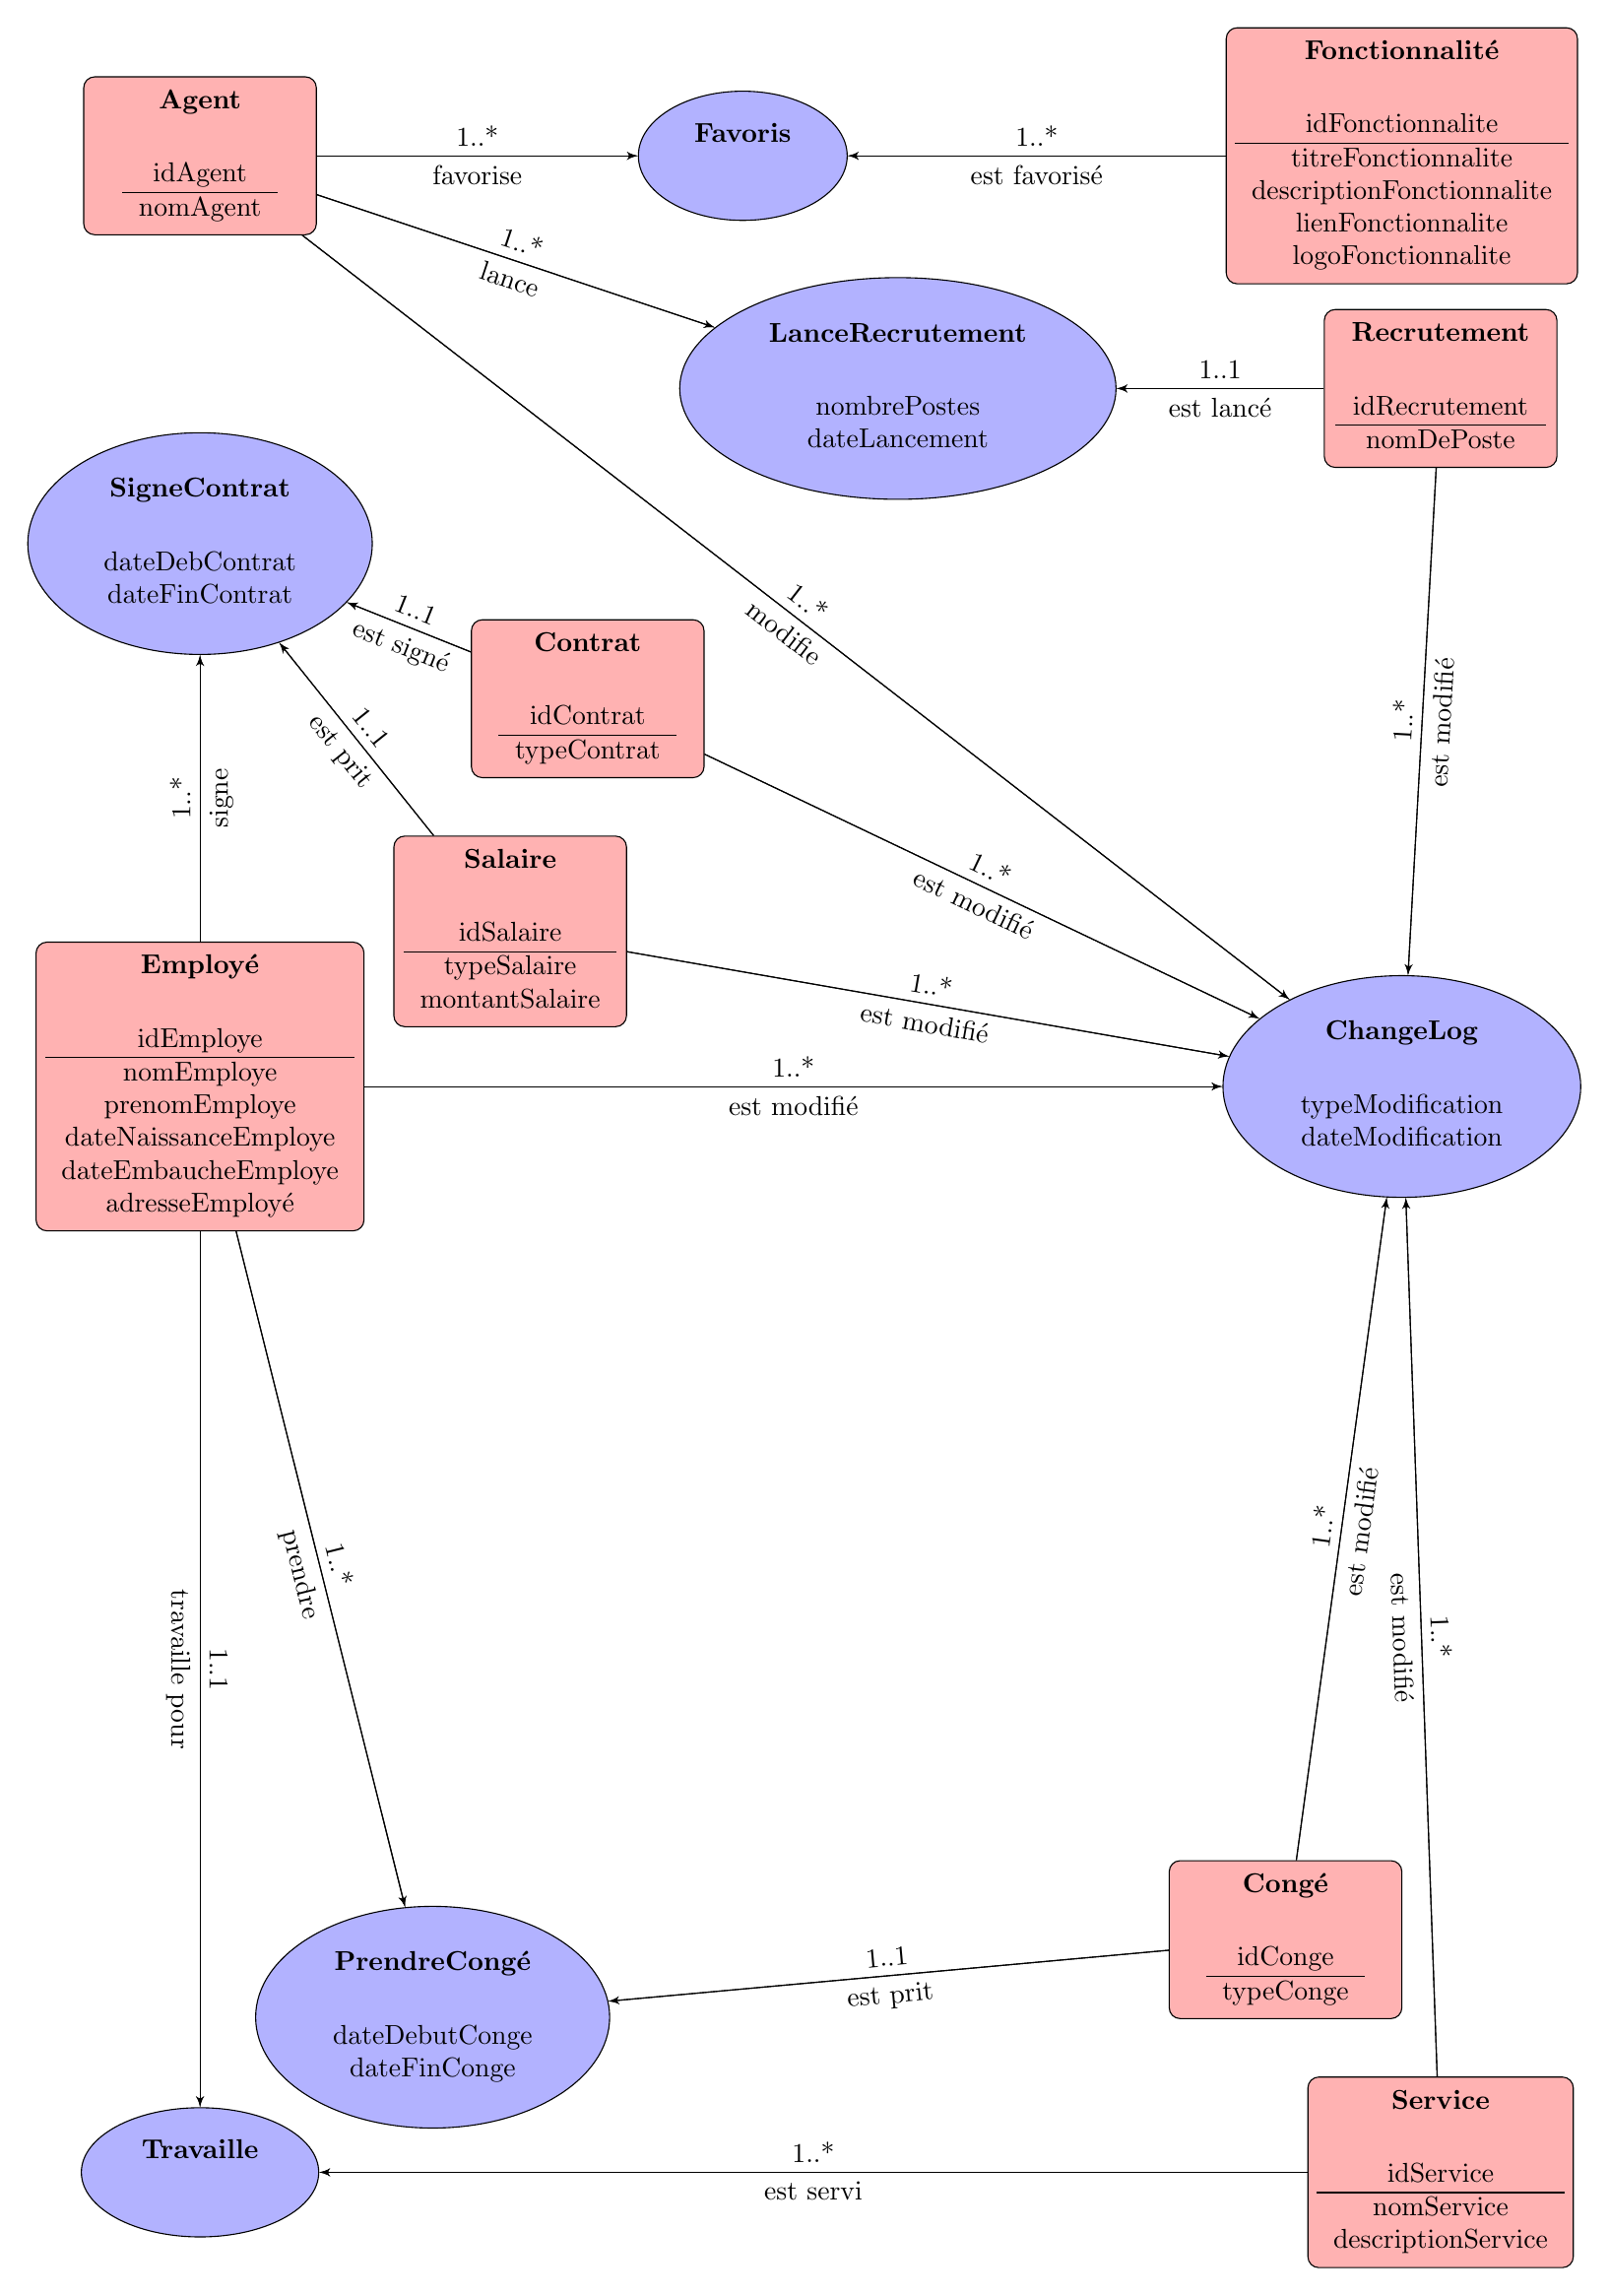
\begin{tikzpicture}[node distance=2cm]

% Entities  
% Gestion des favoris
\node (agent) [entity] {
    \begin{tabular}{c}
        \textbf{Agent} \\ 
        \vspace{0.1cm} \\
        idAgent \\ \hline
        nomAgent\\
        
    \end{tabular}
};
\node (fonctionnalite) [entity, right of=agent, xshift=13.5cm] {
    \begin{tabular}{c}
        \textbf{Fonctionnalité} \\ 
        \vspace{0.1cm} \\
        idFonctionnalite\\ \hline
        titreFonctionnalite\\ 
        descriptionFonctionnalite \\
        lienFonctionnalite \\
        logoFonctionnalite
        
    \end{tabular}
};
%Gestion des tables
\node (employe) [entity, below of=agent, yshift=-10cm] {
    \begin{tabular}{c}
        \textbf{Employé} \\ 
        \vspace{0.1cm} \\
        idEmploye\\ \hline
        nomEmploye\\ 
        prenomEmploye \\
        dateNaissanceEmploye \\
        dateEmbaucheEmploye \\
        adresseEmployé \\
    \end{tabular}
};
\node (service) [entity, below of=employe, yshift=-12cm, xshift=16cm] {
    \begin{tabular}{c}
        \textbf{Service} \\ 
        \vspace{0.1cm} \\
        idService\\ \hline
        nomService\\ 
        descriptionService
    \end{tabular}
};
\node (conge) [entity, above of=service, yshift=1cm, xshift=-2cm] {
    \begin{tabular}{c}
        \textbf{Congé} \\ 
        \vspace{0.1cm} \\
        idConge\\ \hline
        typeConge
    \end{tabular}
};
\node (contrat) [entity, below of=agent, xshift=5cm, yshift=-5cm] {
    \begin{tabular}{c}
        \textbf{Contrat} \\ 
        \vspace{0.1cm} \\
        idContrat\\ \hline
        typeContrat
    \end{tabular}
};
\node (salaire) [entity, below of=agent, xshift=4cm, yshift=-8cm] {
    \begin{tabular}{c}
        \textbf{Salaire} \\ 
        \vspace{0.1cm} \\
        idSalaire\\ \hline
        typeSalaire\\
        montantSalaire
    \end{tabular}
};
\node (recrutement) [entity, right of=agent, xshift=14cm, yshift=-3cm] {
    \begin{tabular}{c}
        \textbf{Recrutement} \\ 
        \vspace{0.1cm} \\
        idRecrutement\\ \hline
        nomDePoste
    \end{tabular}
};

% Relationship
%Gestion des favoris
\node (favoris) [relationship, right of=agent, xshift=5cm] {
    \begin{tabular}{c}
        \textbf{Favoris} \\
        \vspace{0.1cm} \\
        
    \end{tabular}
};
%Gestion des tables
\node (travaille) [relationship, below of=employe, yshift=-12cm] {
    \begin{tabular}{c}
        \textbf{Travaille} \\
        \vspace{0.1cm} \\
        
    \end{tabular}
};
\node (prendreconge) [relationship, below of=employe, yshift=-10cm, xshift=3cm] {
    \begin{tabular}{c}
        \textbf{PrendreCongé} \\
        \vspace{0.1cm} \\
        dateDebutConge\\ 
        dateFinConge\\
    \end{tabular}
};
\node (signecontrat) [relationship, below of=agent, yshift=-3cm] {
    \begin{tabular}{c}
        \textbf{SigneContrat} \\
        \vspace{0.1cm} \\
        dateDebContrat\\
        dateFinContrat
    \end{tabular}
};
\node (lancerecrutement) [relationship, right of=agent, xshift=7cm, yshift=-3cm] {
    \begin{tabular}{c}
        \textbf{LanceRecrutement}\\
        \vspace{0.1cm}\\
        nombrePostes\\
        dateLancement
    \end{tabular}
};
\node (changelog) [relationship, below of=agent, yshift=-10cm, xshift=15.5cm] {
    \begin{tabular}{c}
        \textbf{ChangeLog}\\
        \vspace{0.1cm}\\
        typeModification\\
        dateModification\\
    \end{tabular}
};


% Connections
%Gestion des favoris
\draw [line] (agent) -- node[above, sloped] {1..*}(favoris);
\draw [line] (agent) -- node[below, sloped] {favorise}(favoris);
\draw [line] (fonctionnalite) -- node[above, sloped] {1..*}(favoris);
\draw [line] (fonctionnalite) -- node[below, sloped] {est favorisé}(favoris);
%Gestion des tables
\draw [line] (employe) -- node[above, sloped] {1..1}(travaille);
\draw [line] (employe) -- node[below, sloped] {travaille pour}(travaille);
\draw [line] (service) -- node[above, sloped] {1..*}(travaille);
\draw [line] (service) -- node[below, sloped] {est servi}(travaille);

\draw [line] (employe) -- node[above, sloped] {1..*}(prendreconge);
\draw [line] (employe) -- node[below, sloped] {prendre}(prendreconge);
\draw [line] (conge) -- node[above, sloped] {1..1}(prendreconge);
\draw [line] (conge) -- node[below, sloped] {est prit}(prendreconge);

\draw [line] (employe) -- node[above, sloped] {1..*}(signecontrat);
\draw [line] (employe) -- node[below, sloped] {signe}(signecontrat);
\draw [line] (contrat) -- node[above, sloped] {1..1}(signecontrat);
\draw [line] (contrat) -- node[below, sloped] {est signé}(signecontrat);
\draw [line] (salaire) -- node[above, sloped] {1..1}(signecontrat);
\draw [line] (salaire) -- node[below, sloped] {est prit}(signecontrat);

\draw [line] (agent) -- node[above, sloped] {1..*}(lancerecrutement);
\draw [line] (agent) -- node[below, sloped] {lance}(lancerecrutement);
\draw [line] (recrutement) -- node[above, sloped] {1..1}(lancerecrutement);
\draw [line] (recrutement) -- node[below, sloped] {est lancé}(lancerecrutement);

\draw [line] (agent) -- node[above, sloped] {1..*}(changelog);
\draw [line] (agent) -- node[below, sloped] {modifie}(changelog);
\draw [line] (recrutement) -- node[above, sloped] {1..*}(changelog);
\draw [line] (recrutement) -- node[below, sloped] {est modifié}(changelog);
\draw [line] (salaire) -- node[above, sloped] {1..*}(changelog);
\draw [line] (salaire) -- node[below, sloped] {est modifié}(changelog);
\draw [line] (contrat) -- node[above, sloped] {1..*}(changelog);
\draw [line] (contrat) -- node[below, sloped] {est modifié}(changelog);
\draw [line] (conge) -- node[above, sloped] {1..*}(changelog);
\draw [line] (conge) -- node[below, sloped] {est modifié}(changelog);
\draw [line] (employe) -- node[above, sloped] {1..*}(changelog);
\draw [line] (employe) -- node[below, sloped] {est modifié}(changelog);
\draw [line] (service) -- node[above, sloped] {1..*}(changelog);
\draw [line] (service) -- node[below, sloped] {est modifié}(changelog);

\end{tikzpicture}

\end{document}
